%%%%%%%%%%%%%%%%%%%%%%%%%%%%%%%%%%%%%%%%%%%%%%%%%%%%%%%%%%%%%%%%%%%%%%%%%%%%%%%
\chapter{Power-aware throughput management on multi-core systems}~\label{chap:delta}
%%%%%%%%%%%%%%%%%%%%%%%%%%%%%%%%%%%%%%%%%%%%%%%%%%%%%%%%%%%%%%%%%%%%%%%%%%%%%%%

Power management system have to look at two facets: Power and energy. Servers are
usually limited at the amount of peak power and energy
consumption in order to reduce maintenance cost. Energy and power considerations more often than not accounts 
to the reduction in server space expansion in industries. To combat these constraints, power management systems
use technologies such as dynamic voltage and frequency scaling (DVFS) to reduce peak power
consumption and processor halting such as deep sleep states to conserve energy when idle.
With the advent of virtual machine farms running on a single
server poses the high probability of varied workloads running on a single physical system. 
This element further enhances the requirement of dynamic non-trace driven power management
systems.

Lowering frequency has a pleasant benefit of reducing the power consumption and hence
the energy and cooling costs. But as shown in Chapter~\ref{chap:pds}, Figures~\ref{fig:ipc_speedup} 
and \ref{fig:ipc_epi}, when the average IPC of an application is high, reduction in 
frequency only causes the application to execute for a proportionally longer duration and 
hence having no energy benefit (Figure~\ref{fig:ipc_epi}). The only advantage of reducing
the frequency is the reduction of energy supply into the system per unit time and hence
possibly lower heat dissipation. 

Some power management systems such as \cite{OnDemand} manipulate the DVFS configuration
of the system based on the load. The primary problem with such approaches are not in
their implementation or design, but the fact that there are better power management
systems where the entire processor is powered down during idle time whose power savings are considerably higher than DVFS. 
This brings us to utilizing DVFS mechanisms to conserve power during system \textit{active}
state. 

\cite{AnIntraTask}, \cite{LiveRuntime} and \cite{Phaseaware} propose adapting the clock speed of the the processing element based
on the current application's demand. But this assumes the fact that DVFS transitions
are local to that processor core. Some multi-core processors have dependency between 
processor cores (Transitioning one might potentially transition the other) or systems with 
symmetric multi-threaded features where a single processor
core is visible to the operating system as multiple virtual processors. Thus, applications
executing on such processing elements are tied to each other and any DVFS
transition based on one application might potentially affect another negatively. 

%%%%%%%%%%%%%%%%%%%%%%%%%%%%%%%%%%%%%%%%%%%%%%%%%%%%%%%%%%%%%%%%%%%%%%%%%%%%%%%
\section{Common power management systems}~\label{sec:common_pow}
%%%%%%%%%%%%%%%%%%%%%%%%%%%%%%%%%%%%%%%%%%%%%%%%%%%%%%%%%%%%%%%%%%%%%%%%%%%%%%%

The most popular among power management techniques are load directed systems
which transition a processor to a higher or lower performance state is based on it's current load. Two
of these techniques: \textit{ondemand}\cite{OnDemand} and \textit{conservative} 
were simulated within the existing infrastructure. While the \textit{ondemand}
system raises the performance state to the highest possible level at high loads, but
also reduces the performance state gradually at lower load, the \textit{conservative}
system gradually changes the performance state in either direction. These two are 
shown in Figures \ref{fig:math_ondemand} and \ref{fig:math_conservative}. As both 
are similar in design, only the \textit{ondemand} system was used in the comparison.

\begin{figure}[h!]
\centering
\begin{equation*}
    P_{i}' = \left\{ \begin{array}{lr} 
                   P_{M-1} & : Load \geq 0.8 \\
		   P_{i}-1 & : Load < 0.8
                  \end{array} \right.
\end{equation*}
\caption{The ondemand power management system with M performance states}
\label{fig:math_ondemand}
\end{figure}

\begin{figure}[h!]
\centering
\begin{equation*}
    P_{i}' = \left\{ \begin{array}{lr} 
                   P_{i}+1 & : Load \geq 0.8 \\
		   P_{i}-1 & : Load < 0.8
                  \end{array} \right.
\end{equation*}
\caption{The conservative power management system with M performance states}
\label{fig:math_conservative}
\end{figure}

%%%%%%%%%%%%%%%%%%%%%%%%%%%%%%%%%%%%%%%%%%%%%%%%%%%%%%%%%%%%%%%%%%%%%%%%%%%%%%%
\section{Overview of the Linux cpufreq architecture}~\label{sec:cpufreq}
%%%%%%%%%%%%%%%%%%%%%%%%%%%%%%%%%%%%%%%%%%%%%%%%%%%%%%%%%%%%%%%%%%%%%%%%%%%%%%%

In order to maintain architecture independence, separation of methodology 
and policy, the subsystem in the Linux kernel responsible for managing the 
voltage and frequency configuration separates the procedure into three layers. \textit{cpufreq-drivers}
are responsible for the actual P-State transition and register with the 
intermediate \textit{cpufreq} layer. \textit{cpufreq-governors} are responsible for
policy (How and when to initiate a transition) and also register with the 
\textit{cpufreq} layer. Once a working configuration is initialized, the 
\textit{cpufreq-governor} instructs the \textit{cpufreq-driver} in an indirect
fashion on the required transition. As most of the experimentation mentioned in
this text relates to the AMD Barcelona, the \textit{powernow-k8} \textit{cpufreq-driver}
was used to initiate the transition. 

A \textit{cpufreq} governor \textit{seeker} modeled after the \textit{ondemand} governor
was developed having kernel exported interfaces for the mutator to request transitions. 
A simple registration method was introduced to allow the mutator to be informed 
every time a transition is complete as shown in Figure~\ref{fig:governor}. 
The asynchronous call back mechanism allows the mutator to
update its data structures even when an entity other than itself ( For example, through
the \textit{sysfs} interface) requests for a performance state change. 

\begin{figure}[h!]
  \begin{center}
    %\resizebox{\columnwidth}{!}{
    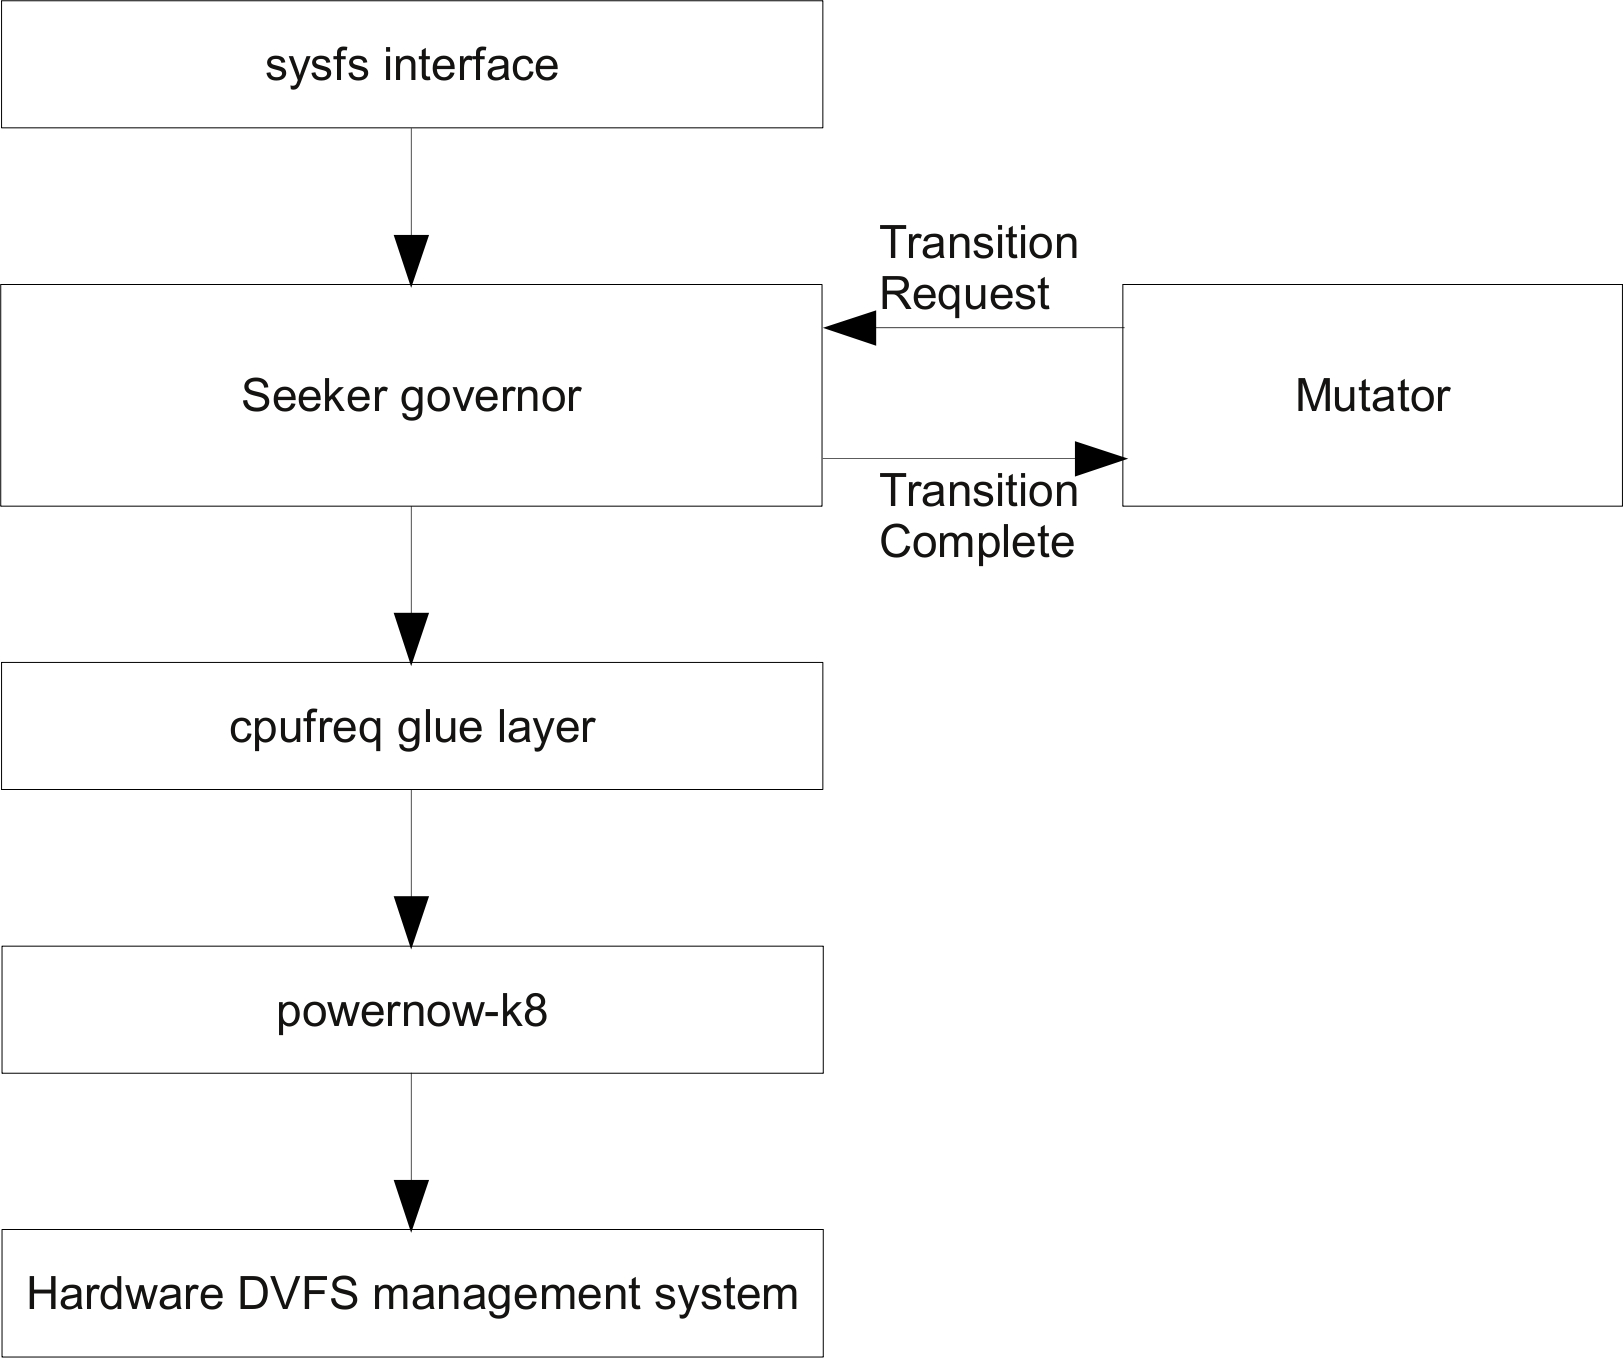
\includegraphics[height=2in]{figures/seeker_governor.jpg}%}
    \caption{The Seeker governor}
    \label{fig:governor}
  \end{center}
\end{figure}

%%%%%%%%%%%%%%%%%%%%%%%%%%%%%%%%%%%%%%%%%%%%%%%%%%%%%%%%%%%%%%%%%%%%%%%%%%%%%%%
\section{Defining the processor layout}~\label{sec:layout}
%%%%%%%%%%%%%%%%%%%%%%%%%%%%%%%%%%%%%%%%%%%%%%%%%%%%%%%%%%%%%%%%%%%%%%%%%%%%%%%

The mutator maintains the layout of the processors $L^m$ as shown in Figure~\ref{fig:mutator_layout_view}
where N is the total number of processors and 
$P_{C_{i}}$ is the performance state at which processor i is currently in. $L^m$
is a vector of length \textit{N} where each element represents the performance state
of the corresponding processor. 
One view of the layout vector $L^s$ was described in Chapter~\ref{chap:pds} 
which was more optimized to view the system of processors as a hierarchal organization
based on their current performance state as the scheduler is designed to be oblivious to individual processors. 
It is clear that both $L^s$ and $L^m$ are different views of the same information and 
the mutator is solely responsible for keeping both consistent. For the rest of this chapter
references to layout or $L$ are with respect to $L^m$. 

\begin{figure}[h!]
\centering
\begin{equation*}
    L^m = [ P_{C_{0}} P_{C_{1}} ... P_{C_{N-1}} ]
\end{equation*}
\caption{Processor layout with N processors}
\label{fig:mutator_layout_view}
\end{figure}


%%%%%%%%%%%%%%%%%%%%%%%%%%%%%%%%%%%%%%%%%%%%%%%%%%%%%%%%%%%%%%%%%%%%%%%%%%%%%%%
\section{The delta constraint}~\label{sec:delta_constraint}
%%%%%%%%%%%%%%%%%%%%%%%%%%%%%%%%%%%%%%%%%%%%%%%%%%%%%%%%%%%%%%%%%%%%%%%%%%%%%%%


It is well known that rapid DVFS transitions can affect the reliability of the system \cite{ImpactDVFS}.
Based on system with a scheduling frequency of \textit{Q} Hz
and \textit{N} processor cores, a per-task demand based DVFS system may potentially cause $Q \times N$ 
DVFS transitions per second. Moore's law predicts the doubling of processor cores every 18 months, implying
future architectures are imposed a linear growth of reliability issues and failure rates with per-task
demand based DVFS systems as proposed in \cite{LiveRuntime} and \cite{Phaseaware}. 

The delta constrained mutation scheme was developed providing the ability to control the rate of transitions
to control the magnitude of mutation allowed every mutation interval thus overcoming the negative effects
of rapid DVFS transitions. Figure~\ref{fig:schedule_mutate} shows the interaction times of these methods. 
The PDS as described in Chapter~\ref{chap:pds} is performed at the resolution of a scheduler quanta, while
the DVFS transitions are performed at a resolution of the mutation interval. In order to have an absolute
upper bound on the DVFS transitions, a parameter called the delta constraint ($\Delta$) was introduced
which limits the maximum number of mutations which can be performed at any particular instant (And hence
limiting the maximum mutations per second to $\frac{\Delta}{\text{Mutation Interval}}$). 

\begin{figure}[h!]
  \begin{center}
    %\resizebox{\columnwidth}{!}{
    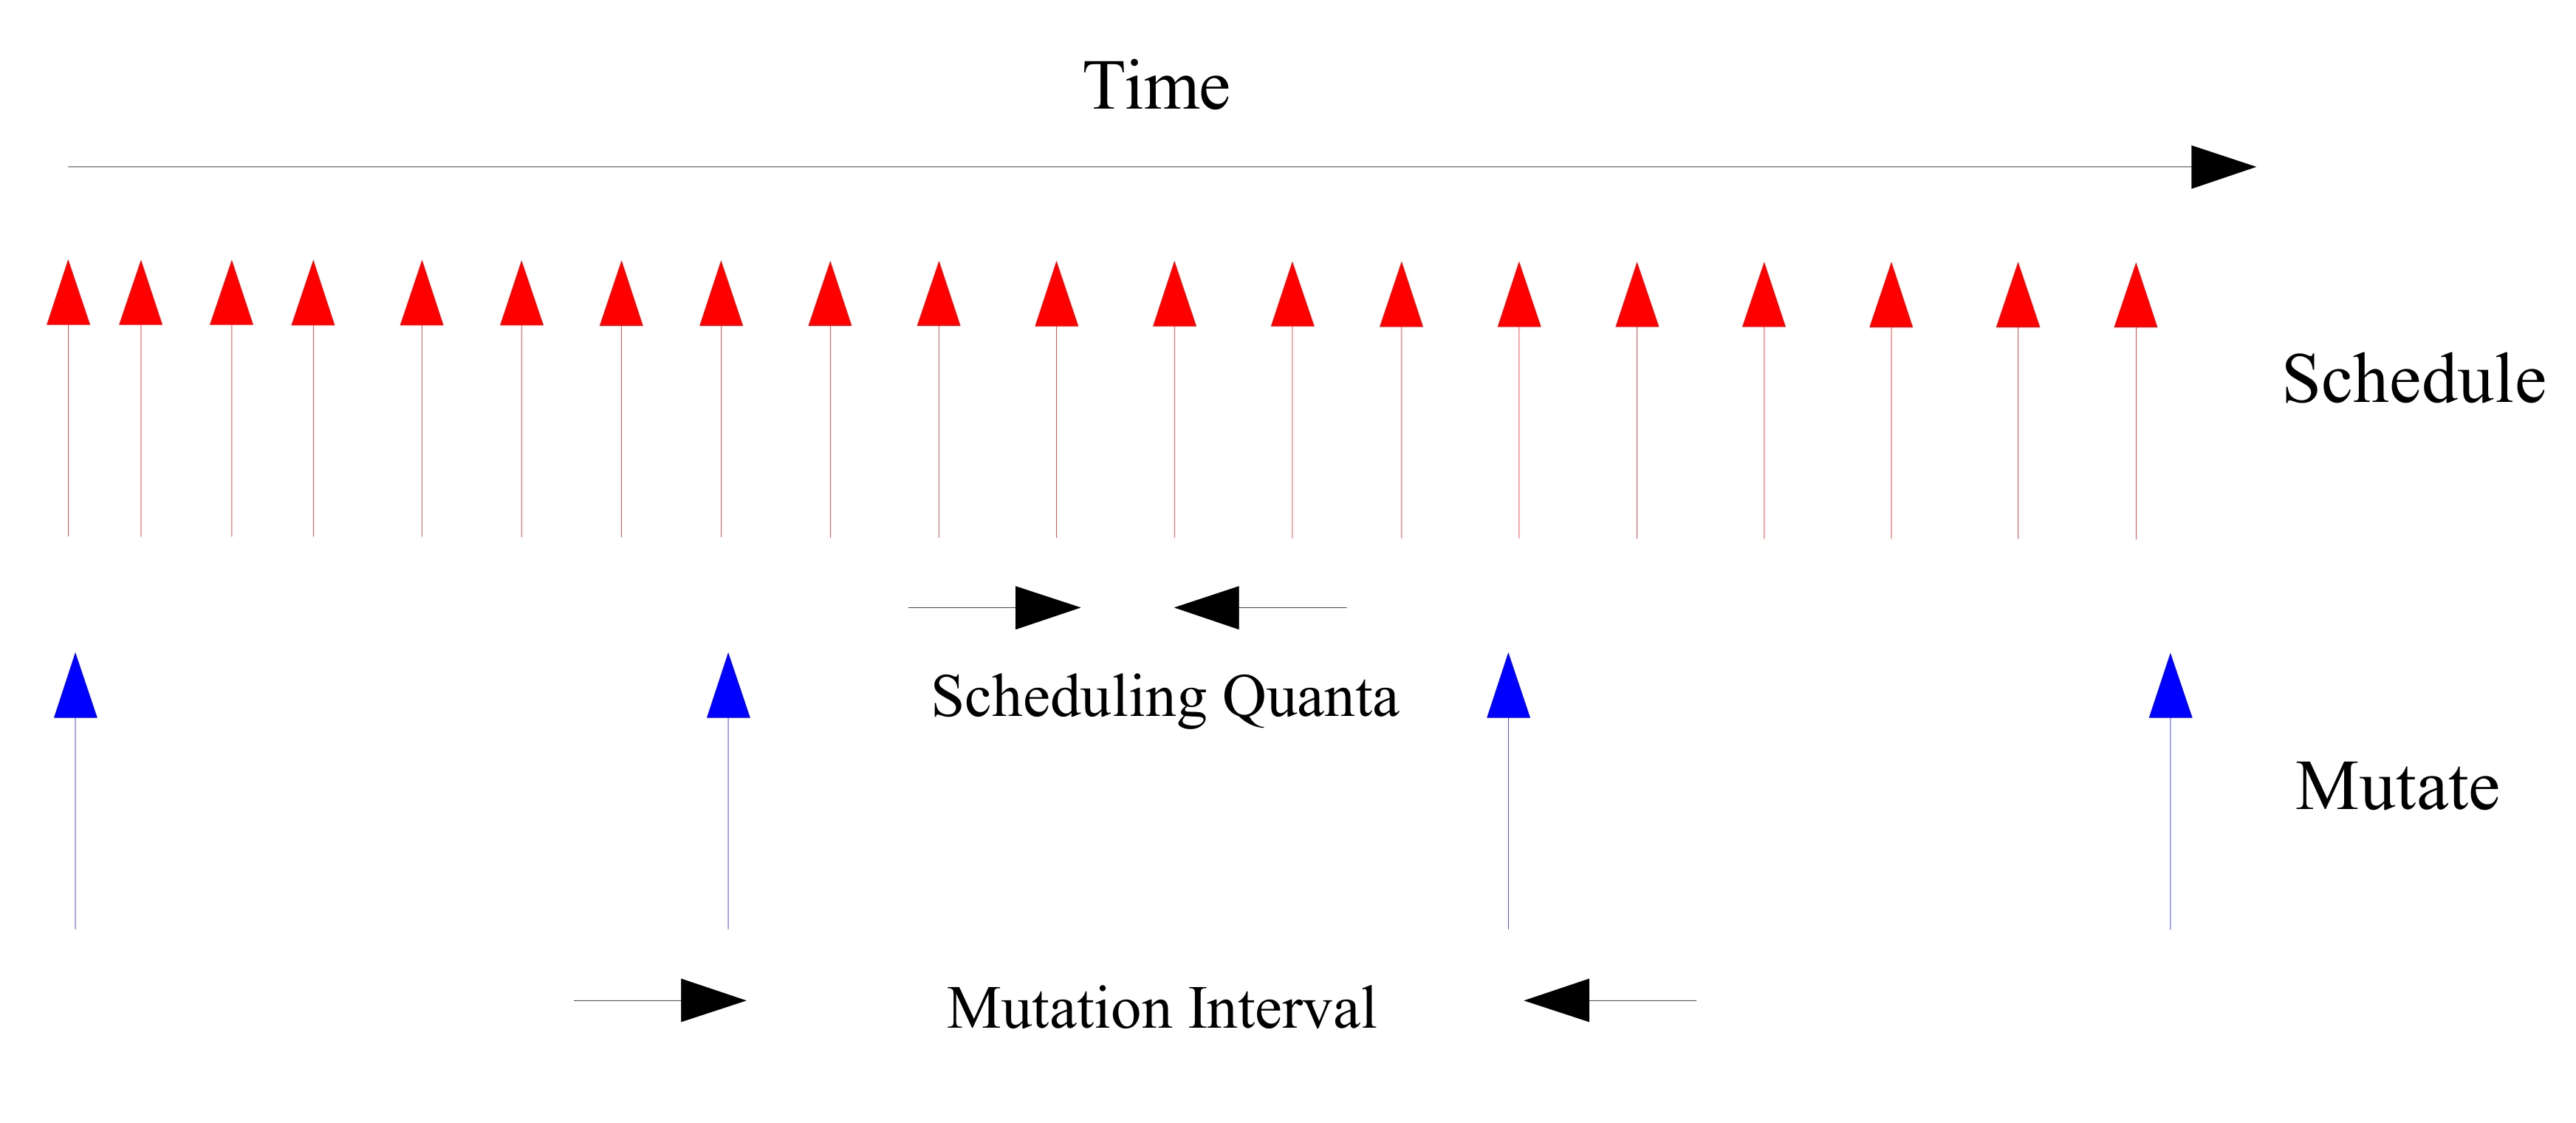
\includegraphics[height=2in]{figures/Schedule_Mutate.jpg}%}
    \caption{Time line comparison of DVFS transitions}
    \label{fig:schedule_mutate}
  \end{center}
\end{figure}


The formal definition is shown in Figure~\ref{fig:Delta_def} where $P_{i}$ is the state of processor \textit{i} 
before a mutation, and $P_{i}'$ is the state of processor \textit{i} after the mutation.
In essence, $\Delta$ is the maximum allowed Manhattan distance by which the processor layout can change. 
Based on this definition, the example mutation provided in Figure~\ref{fig:ex_mutation} has 
a total delta (change) of three and will be allowed for a delta constraint greater than
or equal to 3 ($\Delta \geq 3$).

\begin{figure}[h!]
\centering
\begin{equation*}
    \Delta \geq \displaystyle\sum_{i=0}^{N-1} {| P_{i} - P_{i}' |}
\end{equation*}
\caption{Definition of delta with N processor cores}
\label{fig:Delta_def}
\end{figure}

\begin{figure}[h!]
  \begin{center}
    %\resizebox{\columnwidth}{!}{
    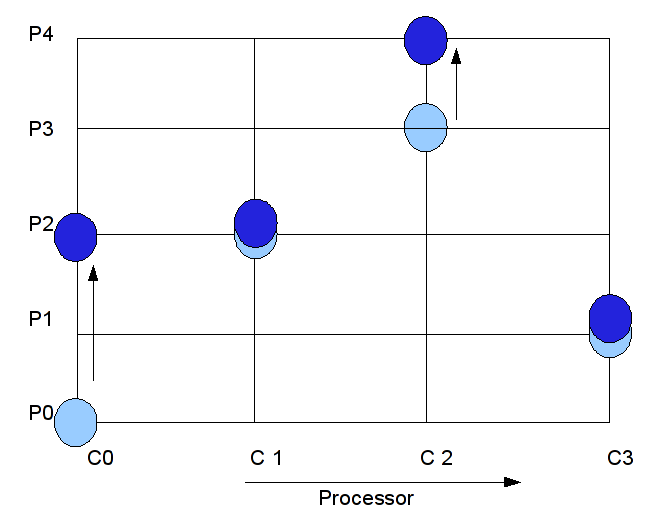
\includegraphics[height=2in]{figures/example_mutation_3.png}%}
    \caption{Example mutation}
    \label{fig:ex_mutation}
  \end{center}
\end{figure}



%%%%%%%%%%%%%%%%%%%%%%%%%%%%%%%%%%%%%%%%%%%%%%%%%%%%%%%%%%%%%%%%%%%%%%%%%%%%%%%
\section{Problem definition}~\label{sec:ago}
%%%%%%%%%%%%%%%%%%%%%%%%%%%%%%%%%%%%%%%%%%%%%%%%%%%%%%%%%%%%%%%%%%%%%%%%%%%%%%%

An overview of the system required is as follows:
\begin{enumerate}
\item The scheduler maintains the demand, a monotonically increasing count of the number
of times each state was requested. 
\item Each processor can take performance states from $0$ to $M-1$. 
\item The total movements: the Manhattan distance from the current layout to the next layout 
should always be less than or equal to the delta constraint. 
\item The system should be partial to maintaining a processors current performance state if such a performance state is requested.
\end{enumerate}

This problem can be expressed as a Multiple choice knapsack problem as shown in Figure~\ref{fig:mckp}, where the capacity of the knapsack 
is the delta constraint, each processor being a variable with multiple choices being the states 
a processor can take. The weight for each choice is the distance that state is from the current 
performance state. It is well understood that such problems are considered NP-Hard.

\begin{figure}[h!]
\centering
\begin{align*}
    & max \displaystyle\sum_{i=0}^{N-1} \displaystyle\sum_{j=0}^{M-1} d_jx_{ij} \\
    & \text{Subject to} : \displaystyle\sum_{i=0}^{N-1} \displaystyle\sum_{j=0}^{M-1} |L_i - j| x_{ij} \leq \delta \\
    & \displaystyle\sum_{j=0}^{M-1} x_{ij} = 1 , i = 0, 1, ..., N-1 \\
    & x_{ij} \in \{0,1\} , i = 0,1,2,...,N-1 ; j = 0,1,2,...,M-1  
\end{align*}
\caption{Problem with N processors each having M states expressed as a multiple choice knapsack problem}
\label{fig:mckp}
\end{figure}

The algorithm provided in \cite{mckp} was implemented and it soon became obvious 
that the algorithm was inefficient for having no concept of transition direction. Thus for 
a delta constraint of 1, if 
the first 3 processors of a quad core system are at state 0 (The lowest performance state),
while the remaining processor is at state 4 (The highest performance state) and the scheduler
demands all the processors to be at state 3: The dynamic programming approach depicted in
\cite{mckp} will transition the forth processor from state 4 to 3 rather than transition 
one of the lower processors closer to state 3. This unfortunately was just one of the examples
among many when the system did not work. This motivated the development of an iterative 
direction based greedy algorithm described below.


%%%%%%%%%%%%%%%%%%%%%%%%%%%%%%%%%%%%%%%%%%%%%%%%%%%%%%%%%%%%%%%%%%%%%%%%%%%%%%%
\section{The delta constrained mutation algorithm}~\label{sec:delta_algo}
%%%%%%%%%%%%%%%%%%%%%%%%%%%%%%%%%%%%%%%%%%%%%%%%%%%%%%%%%%%%%%%%%%%%%%%%%%%%%%%

Figure~\ref{fig:mutation_algo} describes the steps involved in the iterative greedy algorithm. 
Each sub step is described in further sections. The initialization procedure is described in Section~\ref{sec:mut_init}.
Based on the iteration delta constraint $\delta$, a matrix, Manhattan
matrix (\textbf{S}) is constructed and described in Section~\ref{sec:delta_matrix}.
The Manhattan weight vector \textbf{W} is described in Section~\ref{sec:weight}.
The cooperative demand transformation (Creation of the demand field) is described in
\ref{sec:field}. The greedy winning state \textit{w} selection is described in Section~\ref{sec:winner_state}.
The selection of the processor \textit{c} to transition to the winning state \textit{w} 
is described in Section~\ref{sec:winner_proc}. Finally, the parameter adjustments and iteration
termination conditions are described in Section~\ref{sec:param_adjust}. 

\begin{figure}[h!]
  \begin{center}
    %\resizebox{\columnwidth}{!}{
    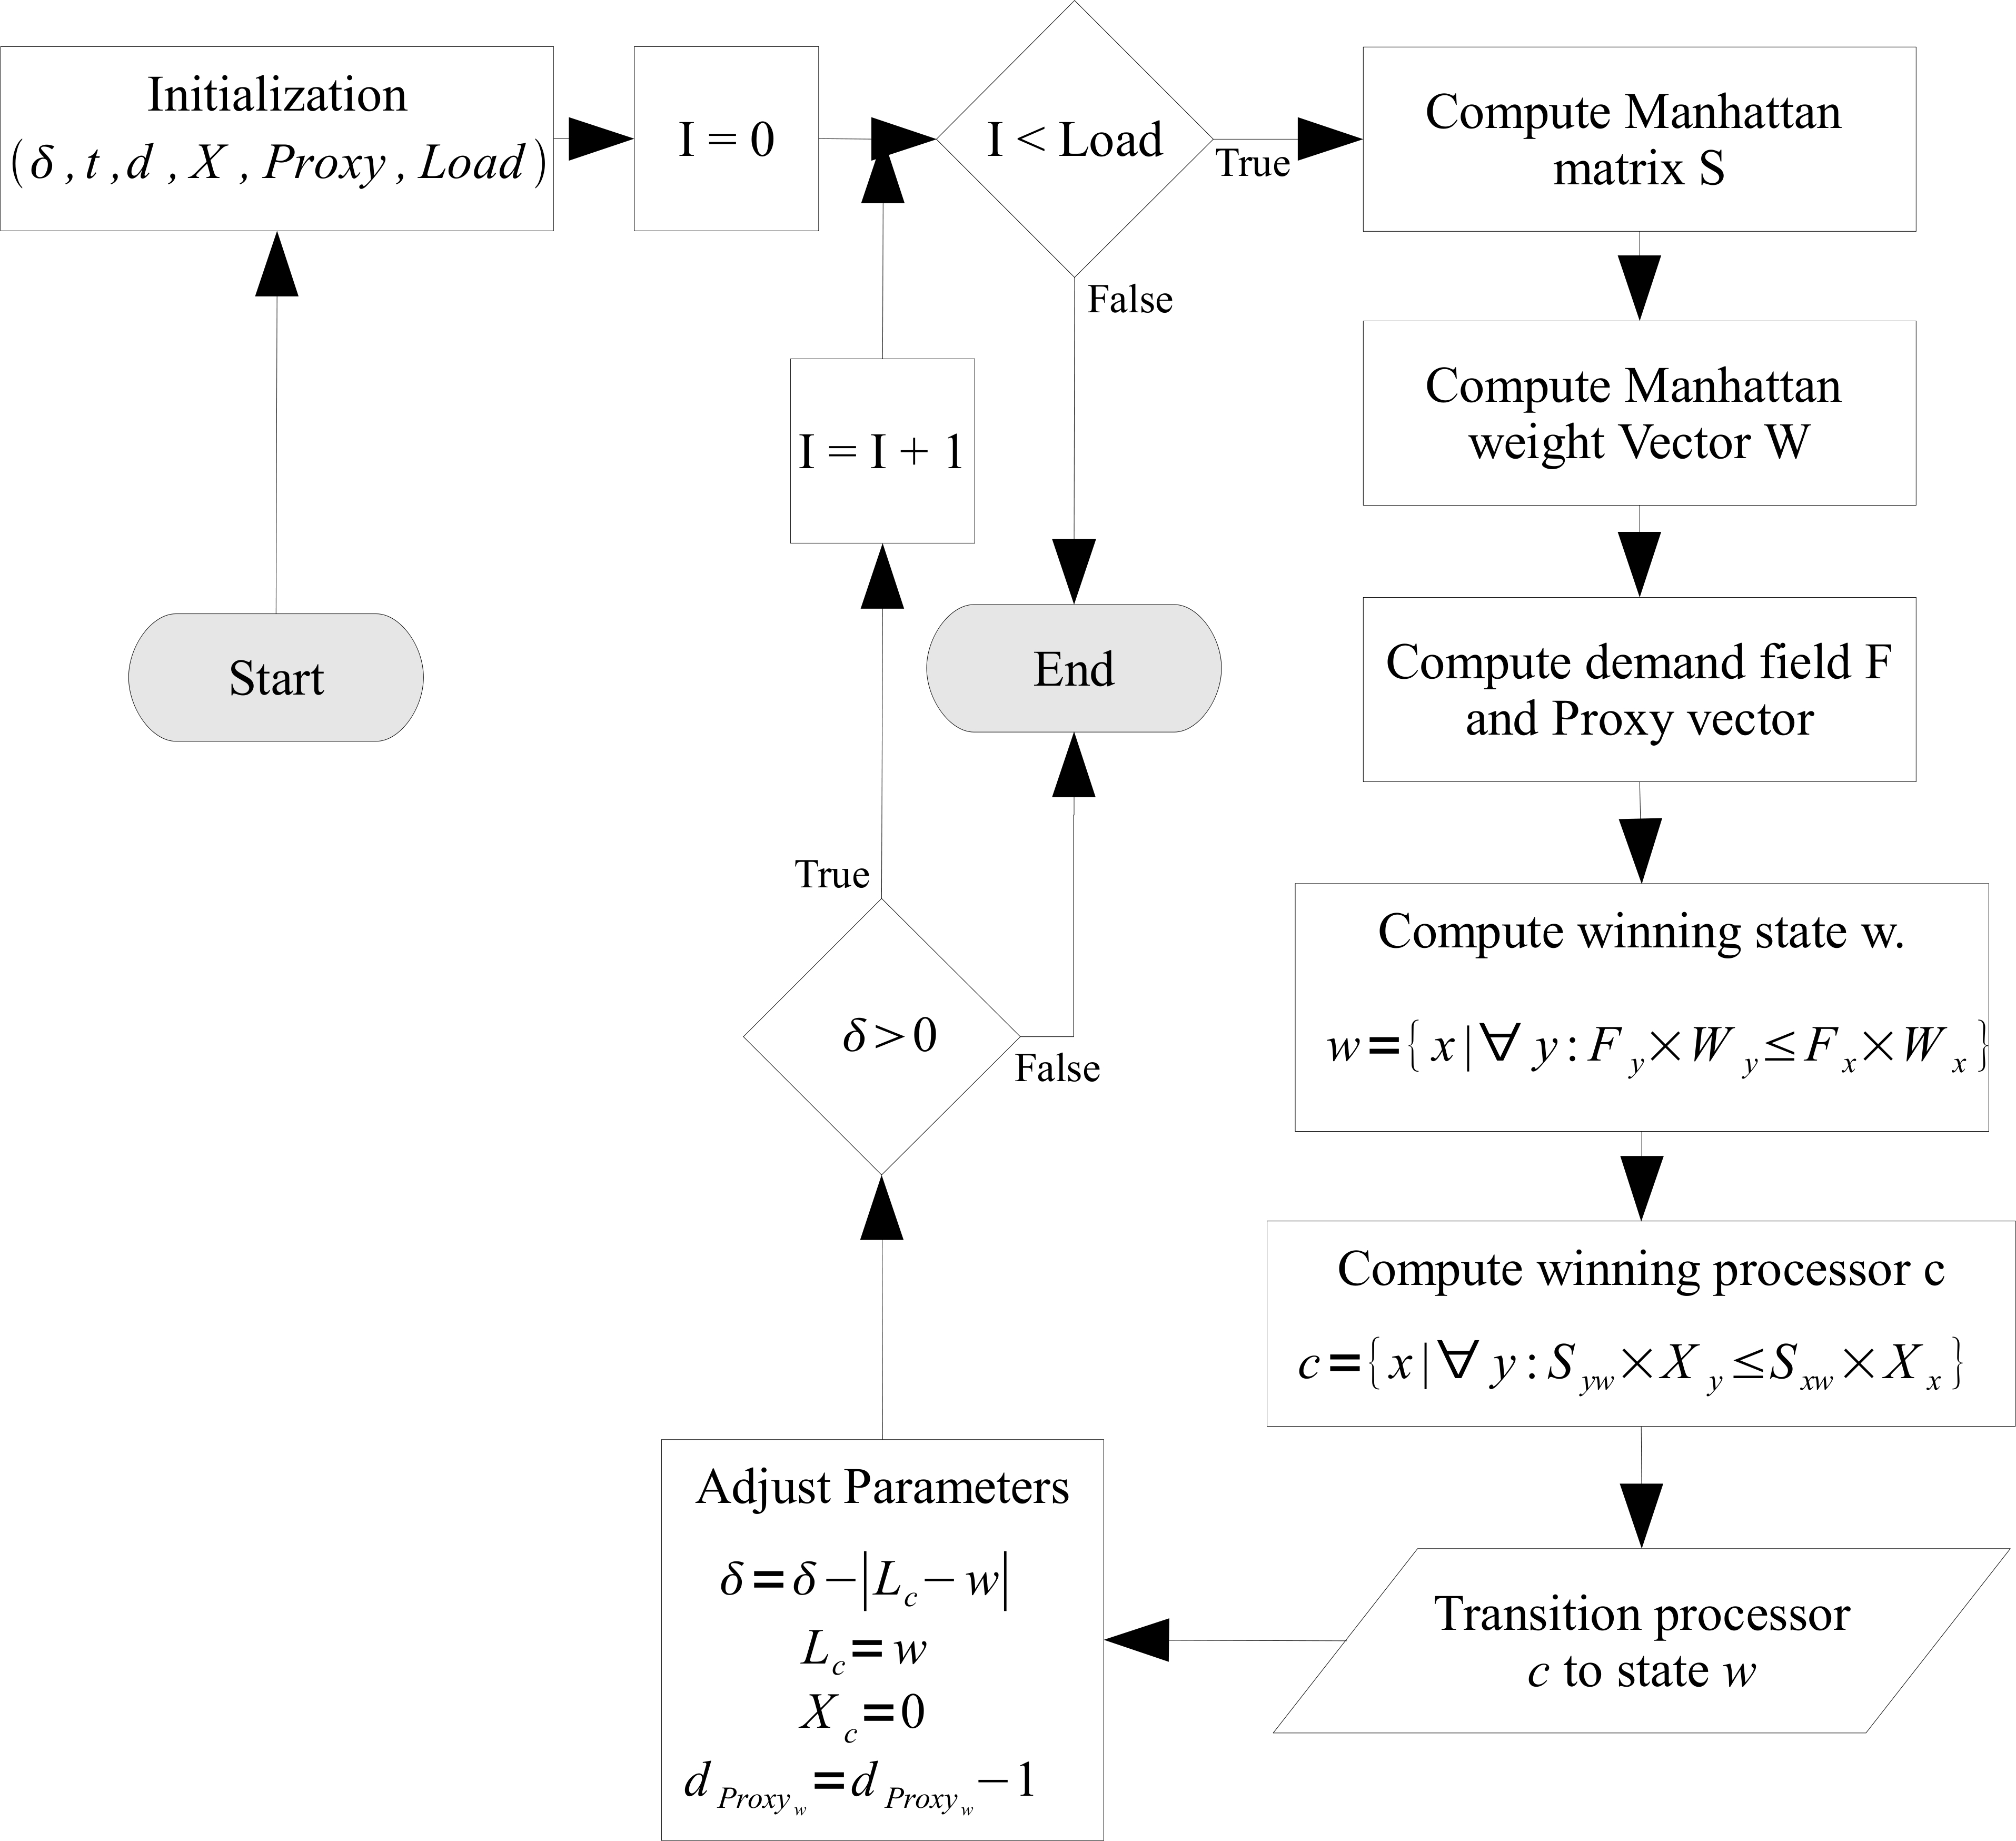
\includegraphics[height=4in]{figures/Mutation_algo.jpg}%}
    \caption{Mutation algorithm}
    \label{fig:mutation_algo}
  \end{center}
\end{figure}

%%%%%%%%%%%%%%%%%%%%%%%%%%%%%%%%%%%%%%%%%%%%%%%%%%%%%%%%%%%%%%%%%%%%%%%%%%%%%%%
\subsection{Initialization}~\label{sec:mut_init}
%%%%%%%%%%%%%%%%%%%%%%%%%%%%%%%%%%%%%%%%%%%%%%%%%%%%%%%%%%%%%%%%%%%%%%%%%%%%%%%

In order to effectively provide only the needed number of processors, the mutator
queries the operating system for the total number of tasks in the ready state $T$. 
From which, the Load of the system in terms of number of processors required is computed 
as shown in Figure~\ref{fig:projected_load}. Using an estimated load based on idle times
of processors was found to be unfruitful as it can be non-representative of the actual 
computing capacity demanded by the number of active tasks. This can be emphasized in situations where multiple
tasks could be queued on a single processor.

\begin{figure}[h!]
\centering
\begin{equation*}
    Load = \left\{
     \begin{array}{lr}
       T & : T \leq N\\
       N & : T > N
     \end{array}
   \right.
\end{equation*}
\caption{Load of the system with N processors and T tasks in the ready state}
\label{fig:projected_load}
\end{figure}

The Performance Directed Scheduler as described in Chapter~\ref{chap:pds} maintains
the demand for each state in the demand vector \textbf{D}. The contents of this vector
cannot be directly consumed as their values pose no direct description of the demand 
of individual performance states. As a direct consequence, vector \textbf{d} is computed based 
on the projected load of the system and the demand vector \textbf{D} and shown in
Figure~\ref{fig:processor_demand}.

\begin{figure}[h!]
\centering
\begin{equation*}
    d_{i} = \frac{D_{i} \times Load}{\displaystyle\sum_{j=0}^{M-1} {D_{j}}}
\end{equation*}
\caption{Processor demand for each performance state in a system with M performance states}
\label{fig:processor_demand}
\end{figure}

$Z_{P}$ and $Z_{R}$, the present and required performance numbers of the system 
are computed as shown in Figure~\ref{fig:Z}. $Z_{P}$ is proportional to the current power drawn by
the system and $Z_{R}$ is proportional to the power required by the performance directed
scheduler in order to optimally satisfy the demands of all running tasks. $Z_{P}$ and $Z_{R}$ 
are further utilized to compute the transition direction, \textit{t} which describes the direction
of transition desired by the system as shown in Figure~\ref{fig:transition_dir}. A transition direction
$t = +1$ implies a higher performance requirement of the layout while a transition direction
$t = -1$ implies a lower performance requirement of the layout. A transition direction equal to zero
implies stability and and mutations must be avoided if possible.

\begin{figure}[h!]
\centering
\begin{equation*}
    Z_{P} = \displaystyle\sum_{i=0}^{N-1} {L_{i}} 
\end{equation*}
\begin{equation*}
    Z_{R} = \displaystyle\sum_{i=0}^{M-1} {i \times d_{i}} 
\end{equation*}
\caption{Current $Z_{P}$ and required $Z_{R}$ performance Number of the system with N processors each of which has M performance states}
\label{fig:Z}
\end{figure}

\begin{figure}[h!]
\centering
\begin{equation*}
    t = \left\{
     \begin{array}{lr}
       1 & : Z_{R} > Z_{P}\\
       0 & : Z_{R} = Z_{P} \\
       -1 & : Z_{R} < Z_{P}
     \end{array}
   \right.
\end{equation*}
\caption{Direction of transition required}
\label{fig:transition_dir}
\end{figure}

Before starting the iterations, the poison vector X is initialized to all ones where
each element corresponds to a processor with a value of 0 implying that the processor
has been allocated a performance state and should not be re-transitioned. 
The iteration delta constraint $\delta$ is initialized to $\Delta$ and shown 
in Figure~\ref{fig:init_X}.

\begin{figure}[h!]
\centering
\begin{equation*}
    \forall i : 0 \geq i < N; X_{i} = 1 
\end{equation*}
\begin{equation*}
    \delta = \Delta
\end{equation*}
\caption{Initialization of the poison vector X and $\delta$ for a system with N processors each capable of M performance states}
\label{fig:init_X}
\end{figure}

%%%%%%%%%%%%%%%%%%%%%%%%%%%%%%%%%%%%%%%%%%%%%%%%%%%%%%%%%%%%%%%%%%%%%%%%%%%%%%%
\subsection{The Manhattan matrix}~\label{sec:delta_matrix}
%%%%%%%%%%%%%%%%%%%%%%%%%%%%%%%%%%%%%%%%%%%%%%%%%%%%%%%%%%%%%%%%%%%%%%%%%%%%%%%

The Manhattan matrix ($N \times T$) is computed with the current values of \textbf{L}, \textbf{d}, and 
$\delta$ as shown in Figure~\ref{fig:delta_mat}. Even though Figure~\ref{fig:delta_mat} seems over 
obfuscated, its purpose and design is quiet simple. A matrix was necessary to provide a weight or value
to each performance state a processor \textit{i} can transition to from its current state $L_i$. The
matrix can best be explained with an example which follows.

\begin{figure}[h!]
\centering
\begin{equation*}
    \forall i,j: 0 \leq i < N, 0 \leq j < T; S_{ij} = \left\{
     \begin{array}{lcr}
       0 & : & j < (L_{i} - \delta) \\
       \frac{T}{2} \times (t^{2} - t + 2) + j - L_{i} & : & (L_{i} - \delta) \leq j < L_{i} \\
       2T & : & j = L_{i}\\
       \frac{T}{2} \times (t^{2} + t + 2) - j + L_{i} & : & L_{i} < j \leq (L_{i} + \delta) \\
       0 & : & j > (L_{i} + \delta)
     \end{array}
   \right.
\end{equation*}
\caption{Manhattan matrix}
\label{fig:delta_mat}
\end{figure}

For example, if the current layout of L = [0,1,2,3] with N, the total number of processors equal to 4 
and M the total number of performance states equal to 5,
the Manhattan matrix \textbf{S} for t = 1, 0 and -1 are shown in Figures~\ref{fig:ex_dmuth}, 
\ref{fig:ex_dmut0} and \ref{fig:ex_dmutl} respectively. 

The Manhattan matrix has \textit{N} rows and \textit{M} columns. Each row in the Manhattan
matrix corresponds to an on-line processor core. Each column corresponds to a performance state
in increasing order. Thus $S_{23}$ corresponds to performance state $P_3$, of processor $C_2$. 

Maximum weight of \textit{2M} is given
to the performance state which processor \textit{i}, is currently in ($L_{i}$).
A weight of 0 is given to states which are forbidden by the iteration delta constraint $\delta$. 
Essentially a weight of 0 is given to states which have a distance from $L_{i}$ greater than $\delta$.

Finally the states allowed by the delta constraint $\delta$, is given a weight lower than
\textit{2M} based on the transition direction \textit{t}. It can be observed from Figure~\ref{fig:ex_dmuth} 
that states higher than the current state $L_{i}$ is tapered down from $2M-1$ while the states
lower than the current state $L_{i}$ is tapered down from $M-1$ giving a greater emphasis to transitions 
which increase the current performance state.

When the transition direction $t = -1$ (Figure~\ref{fig:ex_dmutl}), 
a higher weight is given to the states lower than the current state and hence favoring 
transitioning to a lower performance state. When $t = 0$ (Figure~\ref{fig:ex_dmut0}), 
a transition in either direction is less favorable and hence both sides of $L_{i}$ 
are given equal weights tapered down from $M-1$.


\begin{figure}[h!]
\centering
\begin{equation*}
    S^{t = +1} = \left[
     \begin{array}{ccccc}
       10 & 9 & 0 & 0 & 0 \\
       4 & 10 & 9 & 0 & 0 \\
       0 & 4 & 10 & 9 & 0 \\
       0 & 0 & 4 & 10 & 9
     \end{array}
   \right]
\end{equation*}
\caption{Manhattan matrix \textbf{S}, with t = +1}
\label{fig:ex_dmuth}
\end{figure}

\begin{figure}[h!]
\centering
\begin{equation*}
    S^{t = 0} = \left[
     \begin{array}{ccccc}
       10 & 4 & 0 & 0 & 0 \\
       4 & 10 & 4 & 0 & 0 \\
       0 & 4 & 10 & 4 & 0 \\
       0 & 0 & 4 & 10 & 4
     \end{array}
   \right]
\end{equation*}
\caption{Manhattan matrix \textbf{M}, with t = 0}
\label{fig:ex_dmut0}
\end{figure}

\begin{figure}[h!]
\centering
\begin{equation*}
    S^{t = -1} = \left[
     \begin{array}{ccccc}
       10 & 4 & 0 & 0 & 0 \\
       9 & 10 & 4 & 0 & 0 \\
       0 & 9 & 10 & 4 & 0 \\
       0 & 0 & 9 & 10 & 4
     \end{array}
   \right]
\end{equation*}
\caption{Manhattan matrix \textbf{M}, with t = -1}
\label{fig:ex_dmutl}
\end{figure}

The Manhattan matrix can be viewed as a probability matrix where each each element
$S_{ij}$ indicates the probability that processor \textit{i} can be transitioned to
performance state \textit{j}. The conception of this matrix was achieved by viewing
a probability density function for each processor which was soon modified to its
current definition due to the lack of floating point operations in kernel space 
(Even though possible, the kernel address space does not save the floating point 
context and makes it's use dangerous as the kernel is fully preempt-able).

%%%%%%%%%%%%%%%%%%%%%%%%%%%%%%%%%%%%%%%%%%%%%%%%%%%%%%%%%%%%%%%%%%%%%%%%%%%%%%%
\subsection{The Manhattan weight vector}~\label{sec:weight}
%%%%%%%%%%%%%%%%%%%%%%%%%%%%%%%%%%%%%%%%%%%%%%%%%%%%%%%%%%%%%%%%%%%%%%%%%%%%%%%

The Manhattan weight vector $W$ is constructed as shown in Figure~\ref{fig:state_weight} by summing along each column 
of the Manhattan matrix (projecting the matrix along the columns) and hence
providing an insight of the locality of each state. A higher value of $W_i$ 
indicates a higher probability that there exists active processors in 
performance state \textit{i}. 

\begin{figure}[h!]
\centering
\begin{equation*}
    \forall j: 0 \leq j < M; W_j = \displaystyle\sum_{i=0}^{N-1} {S_{ij}}
\end{equation*}
\caption{The Manhattan weight vector for a system with N processors with each capable of M performance states}
\label{fig:state_weight}
\end{figure}

%%%%%%%%%%%%%%%%%%%%%%%%%%%%%%%%%%%%%%%%%%%%%%%%%%%%%%%%%%%%%%%%%%%%%%%%%%%%%%%
\subsection{Cooperative demand distribution: The demand field}~\label{sec:field}
%%%%%%%%%%%%%%%%%%%%%%%%%%%%%%%%%%%%%%%%%%%%%%%%%%%%%%%%%%%%%%%%%%%%%%%%%%%%%%%

With lower values of $\Delta$, there is a possibility that a state \textit{i}, with 
high demand ($d_i$), might end up with $W_i = 0$ and hence never provided with a processor
in that state. Thus a method was developed in transforming the demand vector \textbf{d}
in such a way that such null performance states cooperatively give up their demand
to the performance state closest to them which has a possibility of being selected. 
This procedure is described in Algorithm~\ref{fig:field}.


%\begin{figure}[h!]
%\centering
\begin{algorithm}[h!]
 \SetLine
 \KwIn{Demand vector \textbf{d}, Manhattan weight vector \textbf{W}}
 \KwOut{Demand field \textbf{F}, Proxy vector \textbf{Proxy}}
 \ForEach{Performance state $i$}{
     $Proxy_i = i$ \;
     $F_i = d_i$ \;
 }
 \ForEach{Performance state $i$}{
   \If{$W_i = 0$ and $d_i > 0$}{
      \If{$t = 1$}{
        $f = max \{ x : x \in N \wedge x < i \wedge W_x > 0 \}$ \;
      }
      \If{$t = -1$}{
        $f = min \{x : x \in N \wedge x > i \wedge W_x > 0 \}$ \;
      }
      \If{$t = 0$}{
        $f = x : x \in N \wedge x \approx i \wedge W_x > 0$ \;
         f is closest to i such that weight $W_f > 0$.
      }
      $F_f = F_f + F_i$ \;
      $F_i = 0$ \;
      $Proxy_f = i$ \;
    }
 }
\caption{Demand field computation}
\label{fig:field}
\end{algorithm}
%\end{figure}


The demand field \textbf{F} is essentially a replicate of \textbf{d}, and differs under
circumstances when for a particular performance state \textit{i}, $W_i = 0$ and $d_i > 0$,
then its demand is distributed to a friend \textit{f} which varies based on the transition
direction t. If transition direction $t = 1$, then the demand is given to the state \textit{f} closest and lesser than
\textit{i} with $W_f > 0$. If the transition direction $t = -1$ then a friend is searched in 
the opposite direction. Finally when $t = 0$, then the closest state \textit{f} to \textit{i} with $W_f > 0$ is chosen as the 
friend. 

In order to track contributions from others, a vector \textbf{Proxy} is maintained indicating 
the source of the demand. Under normal circumstances, $Proxy_i = i$. 

%%%%%%%%%%%%%%%%%%%%%%%%%%%%%%%%%%%%%%%%%%%%%%%%%%%%%%%%%%%%%%%%%%%%%%%%%%%%%%%
\subsection{Greedy performance state selection}~\label{sec:winner_state}
%%%%%%%%%%%%%%%%%%%%%%%%%%%%%%%%%%%%%%%%%%%%%%%%%%%%%%%%%%%%%%%%%%%%%%%%%%%%%%%

Once \textbf{W} and \textbf{F} are computed, performance state \textit{w} is selected
as the winning state when the value of the product $W_w \times F_w$ is the maximum 
for all states \textit{i}. The procedure is mathematically depicted in Figure~\ref{fig:winning_state}.

\begin{figure}[h!]
\centering
\begin{equation*}
    w = {x | \forall y, y \in \mathbb{N} \wedge 0 \leq y < M : W_y \times F_y \leq W_x \times F_x}
\end{equation*}
\caption{Greedy performance state selection for N processors with each having M performance states}
\label{fig:winning_state}
\end{figure}

%%%%%%%%%%%%%%%%%%%%%%%%%%%%%%%%%%%%%%%%%%%%%%%%%%%%%%%%%%%%%%%%%%%%%%%%%%%%%%%
\subsection{Greedy processor selection and transition}~\label{sec:winner_proc}
%%%%%%%%%%%%%%%%%%%%%%%%%%%%%%%%%%%%%%%%%%%%%%%%%%%%%%%%%%%%%%%%%%%%%%%%%%%%%%%

With the winning performance state selected, the processor to be transitioned
is determined by the row \textit{c} in the Manhattan matrix whose value $S_{cw} \times X_c$ 
is maximum and shown in Figure~\ref{fig:winning_proc}. 

Once the selection is made, processor \textit{c} is transitioned to performance state
\textit{w} by invoking the seeker cpufreq governor described in Section~\ref{sec:cpufreq}.

\begin{figure}[h!]
\centering
\begin{equation*}
    c = {x | \forall y, y \in \mathbb{N} \wedge 0 \leq y < N : S_{yw} \times X_y \leq S_{xw} \times X_x}
\end{equation*}
\caption{Greedy processor selection for N processors with each having performance M states}
\label{fig:winning_proc}
\end{figure}

%%%%%%%%%%%%%%%%%%%%%%%%%%%%%%%%%%%%%%%%%%%%%%%%%%%%%%%%%%%%%%%%%%%%%%%%%%%%%%%
\subsection{Parameter change and termination conditions}~\label{sec:param_adjust}
%%%%%%%%%%%%%%%%%%%%%%%%%%%%%%%%%%%%%%%%%%%%%%%%%%%%%%%%%%%%%%%%%%%%%%%%%%%%%%%

Before moving over to the next iteration as shown in Figure~\ref{fig:mutation_algo},
parameters: $\delta$, $L_c$ and $d_p$ are recomputed
as shown in Figure~\ref{fig:adjust}. First as a transition is performed, the iteration delta
must reduce by an equal order and is performed in the first step in Figure~\ref{fig:adjust}.
Next, as processor \textit{c} is no longer in performance state $L_c$, it is updated to
it's new value \textit{w}. Next, as a processor is assigned to performance state \textit{w},
the corresponding demand can be reduced. Finally, the poison vector's position for processor
\textit{c} disabling processor \textit{c} for participating in a transition in a future 
iteration.

This procedure is repeated for \textit{Load} iterations or till the iteration delta coefficient 
$\delta$ reaches 0. Providing the upper bound on the number of iterations as \textit{Load} 
ensures early termination of the iteration when not necessary. 


\begin{figure}[h!]
\centering
\begin{equation*}
    \delta = \delta - |L_{c} - w| 
\end{equation*}
\begin{equation*}
    L_{c} = w 
\end{equation*}
\begin{equation*}
    d_{Proxy_w} = d_{Proxy_w} - 1 
\end{equation*}
\begin{equation*}
    X_c = 0
\end{equation*}
\caption{Iteration parameter change necessary after transitioning processor \textit{c} to performance state \textit{w}}
\label{fig:adjust}
\end{figure}
